\documentclass{article}

\usepackage{neurips_2026}

\usepackage[utf8]{inputenc}
\usepackage[T1]{fontenc}
\usepackage{hyperref}
\usepackage{url}
\usepackage{booktabs}
\usepackage{amsfonts}
\usepackage{nicefrac}
\usepackage{microtype}
\usepackage{xcolor}
\usepackage{graphicx}
\usepackage{amsmath}
\usepackage{float}
\usepackage{hyphenat}

\title{RAGs for Trading: Evaluating Retrieval-Augmented Generation\\
for Structured Financial Signal Analysis}

\author{%
  Ricky Lee \And
  Tarun Badarvada \And
  Dina Barua \\
  CS6180 --- Generative AI
}

\begin{document}

\maketitle

% ================= ABSTRACT =================
\begin{abstract}
Large language models (LLMs) have demonstrated impressive general reasoning capabilities, yet their reliability in strictly rule-governed, structured environments remains an open question. This paper investigates whether Retrieval-Augmented Generation (RAG) improves the decision accuracy and consistency of LLMs applied to a rule-based financial trading strategy. We design three system variants: a zero-shot \textbf{Baseline}, a \textbf{Manual RAG} that injects hand-curated strategy rules into every prompt, and a \textbf{Vector RAG} that dynamically retrieves similar historical trade setups from a ChromaDB vector store. We evaluate all three on 788 labeled historical SPY opening windows. Ground-truth labels are derived from an outcome-window labeler that assesses whether the first five minutes of the NYSE open satisfy a momentum breakout strategy. The Baseline achieves 22.2\% decision accuracy. Manual RAG improves to 25.5\% and Vector RAG reaches 26.1\%. All three systems exhibit a strong PASS-prediction bias and narrowly clustered, overconfident confidence scores. Our results suggest that while RAG provides a consistent, measurable benefit, current instruction-tuned LLMs remain poorly suited for strict rule-following in high-stakes structured domains without additional calibration.
\end{abstract}

% ================= INTRO =================
\section{Introduction}

This paper studies a straightforward question: can a language model reliably follow explicit trading rules in a setting where the correct answer is objectively defined after the fact? LLMs are strong at general instruction following, but they are also prone to producing plausible answers that are not actually grounded in the supplied evidence. In a rule-based financial setting, that failure mode is especially costly.

We picked the NYSE open as our test case because it is one of the most rule-driven windows in trading. In the first five minutes after 9:30 AM, a momentum trader is looking for specific signals: a clean directional breakout, expanding volume, and volatility within an acceptable range. Either those conditions are met or they are not. There is no room for the model to hedge or reinterpret. If it says TAKE on a day that clearly does not qualify, that is a mistake, and in a real account that mistake has a cost.

Retrieval-Augmented Generation is a natural intervention in this setting. Rather than relying on the model to internalize the strategy from pretraining alone, RAG provides the relevant rules or similar historical examples directly at inference time. The goal is to test whether grounded context measurably improves decision quality.

We built three versions of the system. The first is a zero-shot baseline that receives only the raw five-bar SPY opening sequence for that day. The second adds a fixed block of strategy rules to every prompt (Manual RAG). The third dynamically retrieves the most similar historical trading days from a ChromaDB vector store and includes them as context (Vector RAG). All three use \texttt{gpt-4o-mini} and are evaluated on the same 788 labeled test days.

What makes this setting useful for evaluation is that the correct answer is always knowable after the fact. The outcome-window labeler checks whether the price action between 9:35 and 10:30 AM reaches the profit target first, hits the stop first, or does neither by the end of the window, and then collapses that outcome into a binary TAKE or PASS decision for evaluation. This means we are not asking human annotators to judge whether the model's reasoning sounds good. We are checking whether the binary decision the model made matches what the strategy would have actually called for on that day. That is a much stricter test, and it is the right one for this kind of task.

The specific failure mode we were most concerned about is one that is well documented in the LLM literature: a model that produces a confident, fluent explanation that does not actually reference the relevant rules. In a financial context this is particularly problematic, because an explanation that sounds logical can give a trader false confidence in a decision that was never properly grounded. We wanted to know whether RAG reduces this tendency by forcing the model to work from explicit context rather than general intuition.

Our main contributions are:
\begin{enumerate}
    \item A working pipeline comparing a baseline LLM against manual and vector RAG for a structured financial decision task.
    \item A labeled evaluation set of 788 SPY opening windows with objective ground-truth TAKE/PASS labels.
    \item Accuracy, confusion matrix, and confidence distribution results for all three systems.
    \item An analysis of why the accuracy gains were modest and what that tells us about how LLMs handle strict rule-following tasks.
\end{enumerate}

% ================= RELATED WORK =================
\section{Related Work}

\textbf{Retrieval-Augmented Generation (RAG):} Lewis et al.~\cite{lewis2020retrieval} introduced RAG as a method for grounding language model outputs in externally retrieved documents, demonstrating that access to a relevant knowledge base at inference time substantially reduces hallucination. Subsequent work has explored dense passage retrieval \cite{karpukhin2020dense}, iterative retrieval \cite{shi2023replug}, and integration with orchestration frameworks such as LangChain and LlamaIndex. Our work applies these ideas to a structured, rule-based decision task where retrieved context consists of formalized trading rules and labeled historical examples rather than free-text documents.

\textbf{LLM Reasoning in Structured Environments:} A growing body of work highlights limitations of LLMs in tasks requiring strict logical or rule-based reasoning \cite{zhao2023survey}. Models tend to rely on surface-level heuristics and distributional priors rather than faithfully applying supplied rules, especially when those rules conflict with common-sense defaults. This failure mode is directly relevant to financial decision-making, where the correct answer is determined by a fixed formal criterion.

\textbf{Financial Decision Systems:} Existing algorithmic trading infrastructure relies primarily on deterministic rule engines or statistical models. Recent work has explored LLM integration: Lopez-Lira and Tang~\cite{lopez2023can} evaluated GPT-4 on news-based return prediction, and Yu et al.~\cite{yu2023finmem} proposed a memory-augmented LLM trading agent. However, these works focus on sentiment or macroeconomic inputs rather than structured intraday signals and do not evaluate rule-following fidelity under controlled, labeled conditions.

\textbf{Hallucination and Calibration:} The tendency of LLMs to produce overconfident but incorrect outputs is well documented \cite{rawte2023survey, ji2023survey, kadavath2022language}. Kadavath et al.~\cite{kadavath2022language} show that models are frequently miscalibrated, reporting high confidence on incorrect answers. Our results replicate this in a new domain and show that RAG does not substantially improve calibration even when it improves accuracy.

% ================= METHOD =================
\section{Method}

\subsection{System Overview}

We developed a Retrieval-Augmented Generation (RAG) system to evaluate whether retrieval-based context improves LLM decision-making on a structured trading task. The live model input is the five-bar SPY opening sequence from 09:30--09:34 ET. We then compare a baseline model against two retrieval-augmented variants to measure whether explicit rules or similar historical setups improve binary TAKE/PASS decisions.

\subsection{Input Data}

The system uses intraday SPY minute aggregates and VIX minute aggregates sourced from Massive. Each trading day is divided into two windows. The setup window spans 09:30--09:34 ET and consists of five 1-minute SPY bars; this is the only live market sequence shown to the model. The outcome window spans 09:35--10:30 ET and is used only for ground-truth labeling. In addition to the raw SPY bars, we compute engineered features such as gap percentage, first-minute return, net movement, opening range width, volatility, relative volume, and VIX at open. These engineered fields are used for retrieval and analysis, not as the baseline model's primary live input. The entry price is defined as the SPY close at 09:34 ET. Our training and retrieval corpus spans from February 14, 2023 through March 1, 2025. The evaluation period runs from March 2, 2025 through the latest available processed date, maintaining a strict chronological split.

\begin{table}[H]
\centering
\caption{Dataset split summary.}
\label{tab:dataset}
\begin{tabular}{lcc}
\toprule
\textbf{Split} & \textbf{Period} & \textbf{Sessions} \\
\midrule
Training (retrieval corpus) & Feb 14, 2023 -- Mar 1, 2025 & 512 days \\
Test (evaluation)           & Mar 2, 2025 -- present      & 788 days \\
\bottomrule
\end{tabular}
\end{table}

\subsection{Ground-Truth Labeling}

Labels are generated by an outcome-window labeler: a deterministic function that scans price action in the 09:35--10:30 ET window minute by minute and assigns \textbf{TAKE} if the move from the 09:34 entry price hits the strategy's profit target before hitting the stop. If the stop is hit first, the day is labeled \textbf{FAIL\_FAKEOUT}; if neither level is reached by 10:30 ET, the day is labeled \textbf{PASS}. For model evaluation, \textbf{FAIL\_FAKEOUT} is collapsed into the binary \textbf{PASS} class. This makes every label objective and grounded in deterministic strategy logic rather than human judgment.

\subsection{Retrieval Context}

The RAG system retrieves:
\begin{itemize}
    \item Formalized trading strategy rules describing the intended breakout logic.
    \item Labeled historical examples pulled from the training corpus based on similarity to the current day.
\end{itemize}

In the vector setting, each historical document combines the raw five-bar opening sequence with engineered setup features and the historical outcome. These documents are embedded with \texttt{text-embedding-3-small} and stored in a local ChromaDB collection built only from the training period.

\subsection{Model Setup}

We compare three configurations, all using \texttt{gpt-4o-mini} via OpenRouter:
\begin{itemize}
    \item \textbf{Baseline LLM:} Receives only the raw 09:30--09:34 SPY opening bars for the current day. No rules or retrieved examples are included.
    \item \textbf{Manual RAG:} Receives the same raw opening bars plus a fixed strategy-rule block and manually retrieved historical context.
    \item \textbf{Vector RAG:} Receives the same raw opening bars plus top-$k$ similar historical setups retrieved from ChromaDB using \texttt{text-embedding-3-small} embeddings. The ChromaDB index is built from the training period only and never updated during evaluation.
\end{itemize}

\subsection{Output Format}

The model is instructed to produce a fixed three-line text response with:
\begin{itemize}
    \item \textbf{Decision:} TAKE or PASS
    \item \textbf{Confidence Score:} Integer between 0 and 100
    \item \textbf{Explanation:} A short written reason citing the relevant signals or rules
\end{itemize}

This output is parsed into a structured record for evaluation. In the reported results below, all three systems had a 0\% parse error rate across the full evaluation set.

% ================= EXPERIMENTS =================
\section{Experiments}

\subsection{Setup}

We use a chronological train/test split. Historical setups from February 14, 2023 through March 1, 2025 form the retrieval corpus, and held-out evaluation begins on March 2, 2025. The model is evaluated on unseen trading days only. The ChromaDB index is frozen after the training period ends, so test-day outcomes cannot leak into retrieval. All three systems are evaluated on the same 788 test days.

\subsection{Evaluation Metrics}

We evaluate performance using:
\begin{itemize}
    \item \textbf{Accuracy:} the fraction of the 788 test days for which the predicted binary decision matches the ground-truth TAKE/PASS label.
    \item \textbf{Confusion analysis:} how often the model predicts TAKE versus PASS and where those decisions fail.
    \item \textbf{Confidence distribution:} the range and concentration of self-reported confidence scores and whether they align with correctness.
\end{itemize}

% ================= RESULTS =================
\section{Results}

\subsection{Decision Accuracy}

Table~\ref{tab:results} reports decision accuracy and related statistics for all three systems. RAG augmentation yields consistent accuracy improvements in both configurations. Vector RAG achieves the highest accuracy at 26.1\%, a 3.9 percentage point improvement over the 22.2\% baseline. Manual RAG reaches 25.5\%, confirming that explicit rule injection alone provides measurable benefit. The marginal gap between Manual RAG and Vector RAG (0.6 pp) indicates that dynamic retrieval of historical analogues adds a small but consistent signal beyond static rule grounding.

\begin{table}[H]
\centering
\caption{Evaluation results on the 788-instance test set. All parse error rates are 0.0\%.}
\label{tab:results}
\begin{tabular}{lcccc}
\toprule
\textbf{Model} & \textbf{Accuracy} & \textbf{Correct (n)} & \textbf{Conf.\ Range} & \textbf{vs.\ Baseline} \\
\midrule
Baseline LLM   & 22.2\% & 175 & 70--85 & --- \\
Manual RAG     & 25.5\% & 201 & 75--85 & +3.3 pp \\
Vector RAG     & 26.1\% & 206 & 75--85 & +3.9 pp \\
\bottomrule
\end{tabular}
\end{table}

\begin{figure}[H]
  \centering
  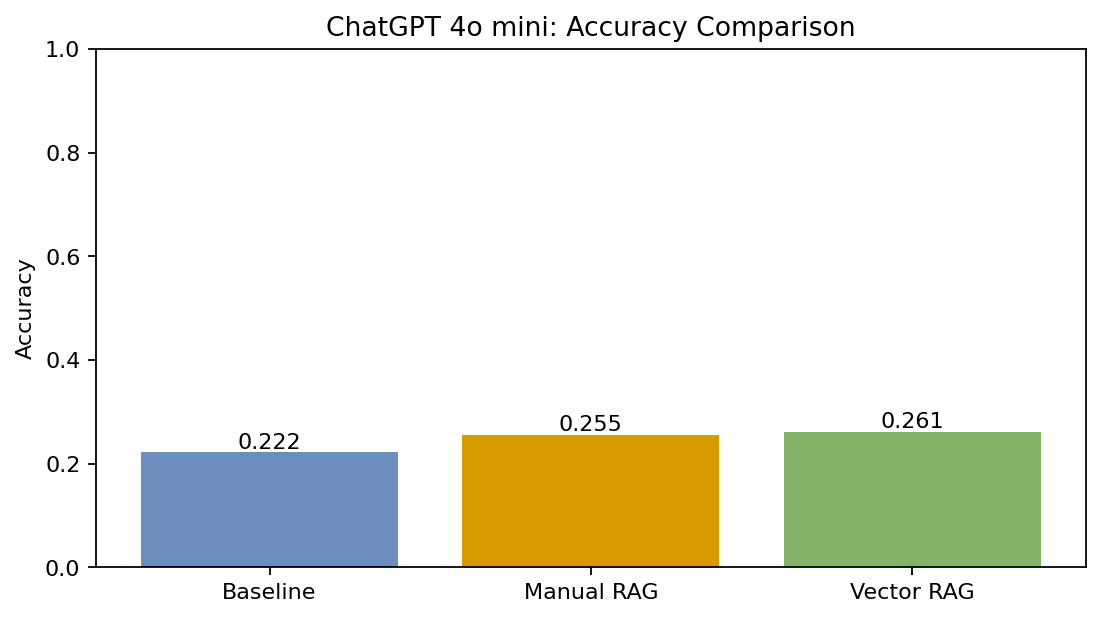
\includegraphics[width=0.72\linewidth]{data/generated/plots/chatgpt_4o_mini_accuracy_comparison.png}
  \caption{Decision accuracy comparison across all three system configurations on the 788-instance test set.}
  \label{fig:accuracy}
\end{figure}

\subsection{Correct versus Wrong Predictions}

Figure~\ref{fig:correct_wrong} shows absolute counts of correct and incorrect decisions per system. All three produce far more wrong decisions than correct ones over the 788-session period. Manual RAG and Vector RAG each recover approximately 25 to 30 additional correct predictions relative to the baseline.

\begin{figure}[H]
  \centering
  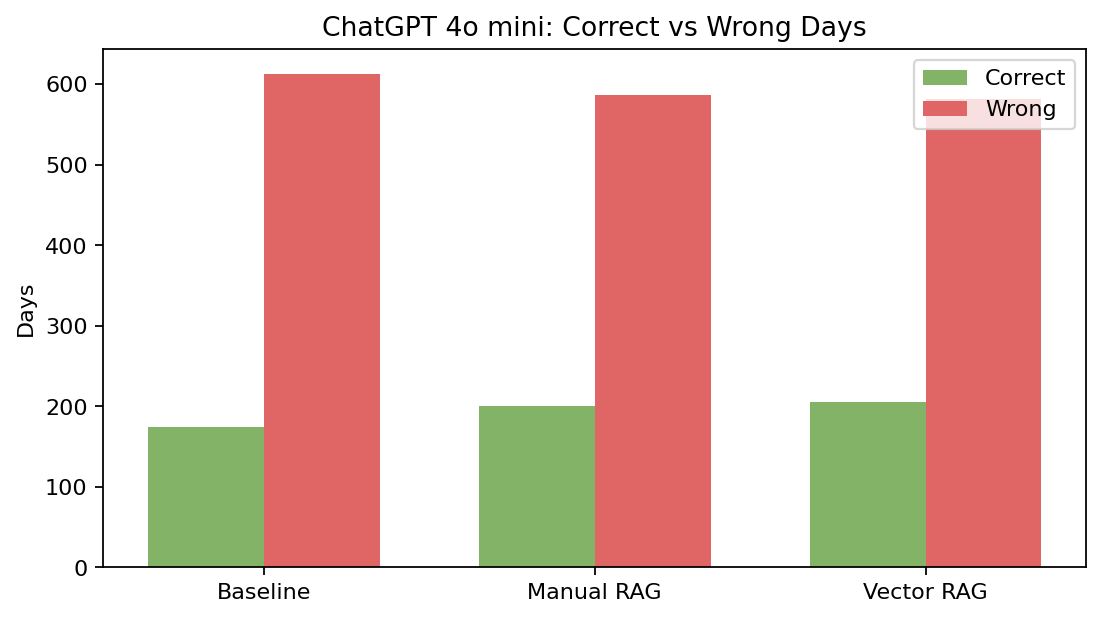
\includegraphics[width=0.72\linewidth]{data/generated/plots/chatgpt_4o_mini_correct_vs_wrong_days.png}
  \caption{Absolute count of correct (green) and wrong (red) decisions per system across 788 test sessions.}
  \label{fig:correct_wrong}
\end{figure}

\subsection{Confusion Matrix Analysis}

Figure~\ref{fig:confusion} shows confusion matrices for all three systems. A strong and consistent PASS-prediction bias is visible across all configurations. TAKE recall is low in every case. Manual RAG is the most conservative, predicting TAKE on the fewest days. Vector RAG shows slightly more balanced TAKE predictions, suggesting that exposure to labeled historical TAKE examples nudges the model toward identifying valid setups.

\begin{figure}[H]
  \centering
  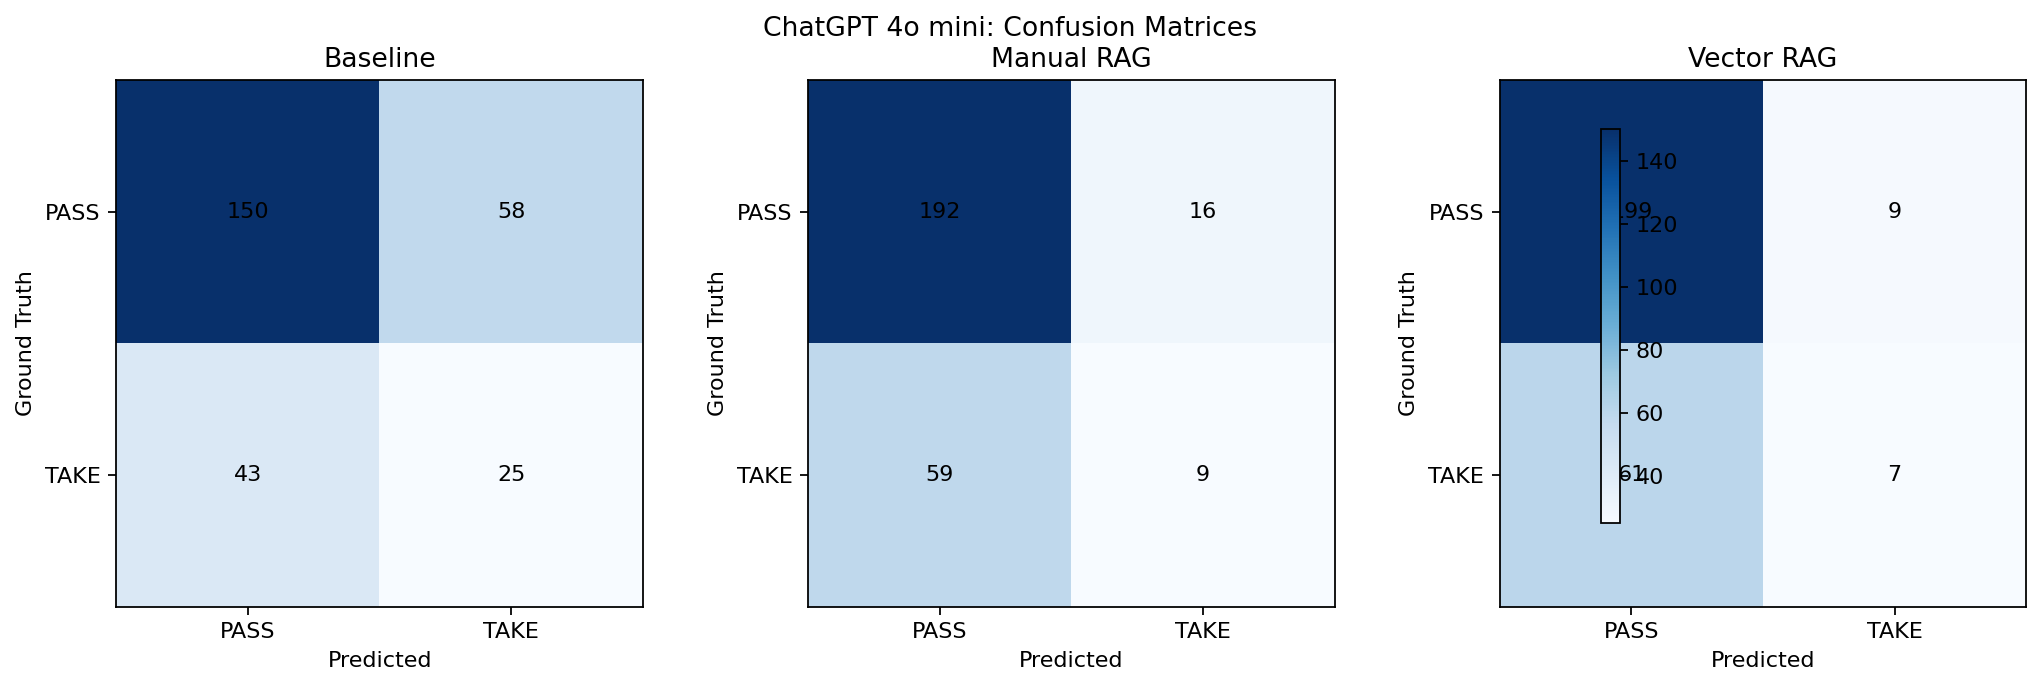
\includegraphics[width=\linewidth]{data/generated/plots/chatgpt_4o_mini_confusion_matrices.png}
  \caption{Confusion matrices for Baseline (left), Manual RAG (center), and Vector RAG (right). All three systems exhibit a pronounced PASS-prediction bias with low TAKE recall.}
  \label{fig:confusion}
\end{figure}

\subsection{Confidence Calibration}

Figure~\ref{fig:confidence} shows the distribution of self-reported confidence scores. All three systems concentrate their scores in a narrow 70 to 85 band regardless of whether the decision is correct or incorrect. High reported confidence is therefore not predictive of correctness, which is a calibration failure consistent with prior findings on instruction-tuned LLMs \cite{kadavath2022language}.

\begin{figure}[H]
  \centering
  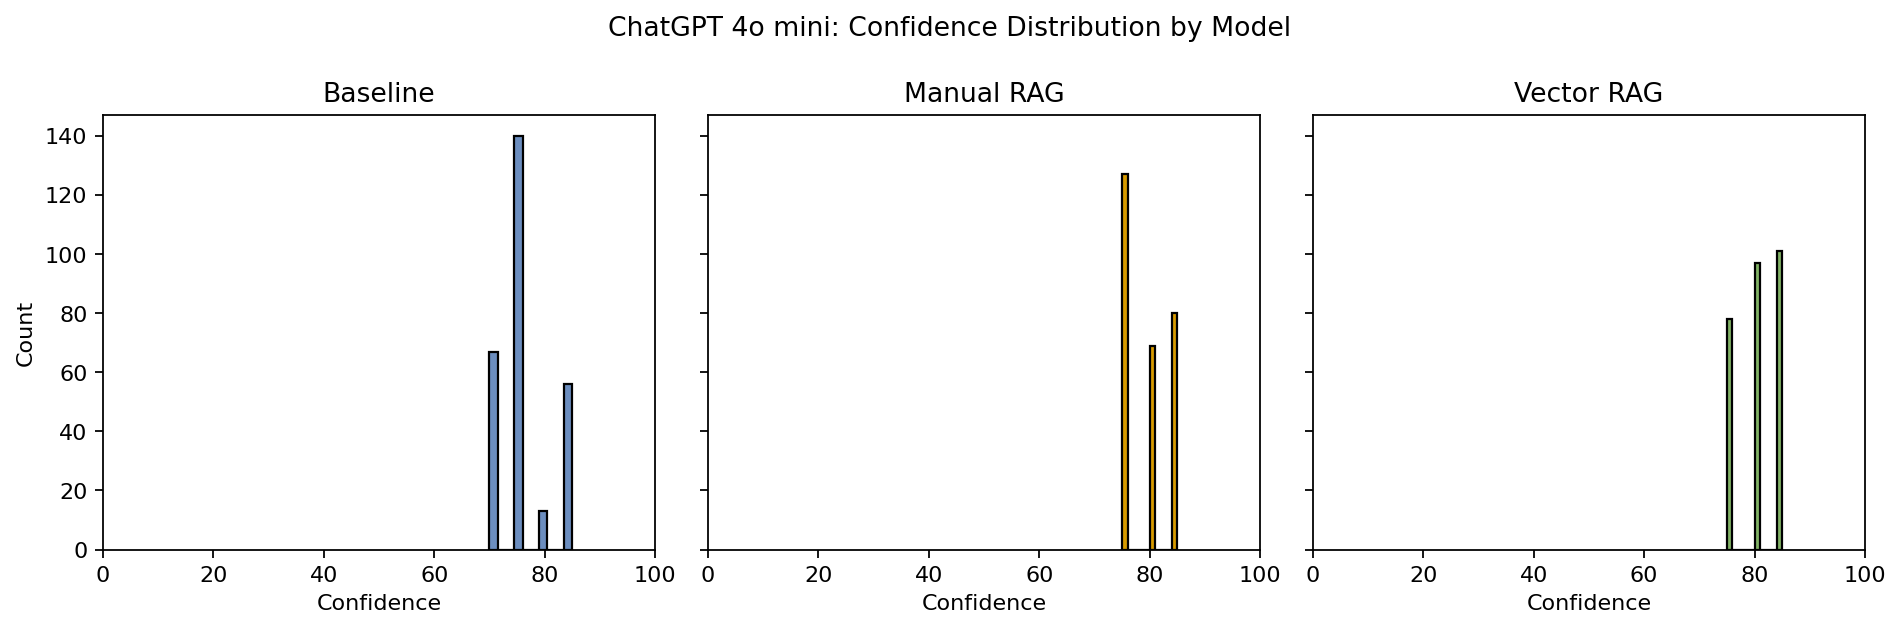
\includegraphics[width=\linewidth]{data/generated/plots/chatgpt_4o_mini_confidence_histograms.png}
  \caption{Confidence score distributions for Baseline (left), Manual RAG (center), and Vector RAG (right). All three systems report confidence in the 70 to 85 range irrespective of correctness, indicating systematic overconfidence.}
  \label{fig:confidence}
\end{figure}

% ================= DISCUSSION =================
\section{Discussion}

RAG did help. Both versions beat the baseline and the improvement was consistent. However, the overall accuracy range of 22 to 26\% is still low, and there are several plausible reasons.

First, the task is genuinely hard. The first five minutes of the NYSE open are noisy, and the five-minute signal window does not always predict what happens in the outcome window cleanly. Even a human trader following the same rules would not get it right every time.

Second, the model has a strong default toward PASS. Looking at the confusion matrices, all three systems miss most of the TAKE days. Part of this is probably because PASS days outnumber TAKE days in the test set. A strategy with strict entry criteria naturally fires rarely. But it also looks like the model is just being conservative when uncertain, which means it avoids false alarms but misses real setups.

Third, confidence scores are essentially useless here. Every model reports 70 to 85\% confidence whether it is right or wrong. This is a known issue with instruction-tuned LLMs but it is especially visible in our results. In a real trading context, you would want to know when the model is uncertain, and these scores do not tell you that.

The Vector RAG's slight edge over Manual RAG suggests that seeing similar historical days helps a little, but the retrieved examples are based on feature similarity, not outcome similarity. Two days can look similar in terms of gap, volume, and range but play out very differently. Better retrieval, such as filtering by outcome or using a learned similarity function, could help here.

% ================= LIMITATIONS =================
\section{Limitations}

This study has several limitations. First, the dataset is limited to SPY intraday data, which may not generalize to other assets or timeframes. Second, the system does not operate in a live trading environment and does not account for real-world constraints such as latency or slippage. Third, we only tested one model (\texttt{gpt-4o-mini}) and did not vary the number of retrieved examples or try other retrieval strategies. Finally, the evaluation focuses on decision accuracy. We did not manually check whether the model's written explanations actually referenced the right rules, which was originally something we wanted to measure.

% ================= CONCLUSION =================
\section{Conclusion}

We tested whether RAG improves LLM decision-making on a rule-based financial trading task. Using 788 labeled SPY opening windows, we found that both RAG configurations outperformed the baseline. Vector RAG reached 26.1\% accuracy versus 22.2\% for the baseline, with Manual RAG at 25.5\%. The improvement is real and consistent, but modest.

The bigger takeaway is that all three systems struggled with the same problems: a PASS bias, low TAKE recall, and overconfident scores that do not track correctness. RAG helps the model make better use of the available context, but it does not fix the underlying tendency of LLMs to play it safe and report false confidence. For a setting like this one, where getting the TAKE days right actually matters, that is a significant limitation worth building on in future work.

% ================= REFERENCES =================
\bibliographystyle{plain}
\begin{thebibliography}{99}

\bibitem{karpukhin2020dense}
V. Karpukhin, B. Oguz, S. Min, P. Lewis, L. Wu, S. Edunov, D. Chen, and W. Yih.
Dense passage retrieval for open-domain question answering.
In \textit{Proceedings of EMNLP}, 2020.

\bibitem{kadavath2022language}
S. Kadavath, T. Conerly, A. Askell, et al.
Language models (mostly) know what they know.
\textit{arXiv preprint arXiv:2207.05221}, 2022.

\bibitem{lewis2020retrieval}
P. Lewis, E. Perez, A. Piktus, F. Petroni, V. Karpukhin, N. Goyal, H. K\"{u}ttler,
M. Lewis, W. Yih, T. Rockt\"{a}schel, S. Riedel, and D. Kiela.
Retrieval-augmented generation for knowledge-intensive NLP tasks.
In \textit{Proceedings of NeurIPS}, 2020.

\bibitem{lopez2023can}
A. Lopez-Lira and Y. Tang.
Can ChatGPT forecast stock price movements?
\textit{arXiv preprint arXiv:2304.07619}, 2023.

\bibitem{ji2023survey}
Z. Ji, N. Lee, R. Frieske, T. Yu, D. Su, Y. Xu, E. Ishii, Y. Bang, A. Madotto, and P. Fung.
Survey of hallucination in natural language generation.
\textit{ACM Computing Surveys}, 55(12):1--38, 2023.

\bibitem{rawte2023survey}
V. Rawte, A. Sheth, and A. Das.
A survey of hallucination in large foundation models.
\textit{arXiv preprint arXiv:2309.05922}, 2023.

\bibitem{shi2023replug}
W. Shi, S. Min, M. Yasunaga, M. Seo, R. James, M. Lewis, L. Zettlemoyer, and W. Yih.
REPLUG: Retrieval-augmented language model pre-training.
\textit{arXiv preprint arXiv:2301.12652}, 2023.

\bibitem{yu2023finmem}
S. Yu, H. Li, W. Wang, Y. Yang, and K. Zhang.
FinMem: A performance-enhanced LLM trading agent with layered memory and character design.
\textit{arXiv preprint arXiv:2311.13743}, 2023.

\bibitem{zhao2023survey}
W. X. Zhao, K. Zhou, J. Li, et al.
A survey of large language models.
\textit{arXiv preprint arXiv:2303.18223}, 2023.

\end{thebibliography}

\newpage
\input{checklist.tex}

\end{document}
